% Options for packages loaded elsewhere
\PassOptionsToPackage{unicode}{hyperref}
\PassOptionsToPackage{hyphens}{url}
%
\documentclass[
  ignorenonframetext,
]{beamer}
\usepackage{pgfpages}
\setbeamertemplate{caption}[numbered]
\setbeamertemplate{caption label separator}{: }
\setbeamercolor{caption name}{fg=normal text.fg}
\beamertemplatenavigationsymbolsempty
% Prevent slide breaks in the middle of a paragraph
\widowpenalties 1 10000
\raggedbottom
\setbeamertemplate{part page}{
  \centering
  \begin{beamercolorbox}[sep=16pt,center]{part title}
    \usebeamerfont{part title}\insertpart\par
  \end{beamercolorbox}
}
\setbeamertemplate{section page}{
  \centering
  \begin{beamercolorbox}[sep=12pt,center]{part title}
    \usebeamerfont{section title}\insertsection\par
  \end{beamercolorbox}
}
\setbeamertemplate{subsection page}{
  \centering
  \begin{beamercolorbox}[sep=8pt,center]{part title}
    \usebeamerfont{subsection title}\insertsubsection\par
  \end{beamercolorbox}
}
\AtBeginPart{
  \frame{\partpage}
}
\AtBeginSection{
  \ifbibliography
  \else
    \frame{\sectionpage}
  \fi
}
\AtBeginSubsection{
  \frame{\subsectionpage}
}
\usepackage{amsmath,amssymb}
\usepackage{lmodern}
\usepackage{ifxetex,ifluatex}
\ifnum 0\ifxetex 1\fi\ifluatex 1\fi=0 % if pdftex
  \usepackage[T1]{fontenc}
  \usepackage[utf8]{inputenc}
  \usepackage{textcomp} % provide euro and other symbols
\else % if luatex or xetex
  \usepackage{unicode-math}
  \defaultfontfeatures{Scale=MatchLowercase}
  \defaultfontfeatures[\rmfamily]{Ligatures=TeX,Scale=1}
\fi
\usetheme[]{Copenhagen}
\usecolortheme{dolphin}
\usefonttheme{structurebold}
% Use upquote if available, for straight quotes in verbatim environments
\IfFileExists{upquote.sty}{\usepackage{upquote}}{}
\IfFileExists{microtype.sty}{% use microtype if available
  \usepackage[]{microtype}
  \UseMicrotypeSet[protrusion]{basicmath} % disable protrusion for tt fonts
}{}
\makeatletter
\@ifundefined{KOMAClassName}{% if non-KOMA class
  \IfFileExists{parskip.sty}{%
    \usepackage{parskip}
  }{% else
    \setlength{\parindent}{0pt}
    \setlength{\parskip}{6pt plus 2pt minus 1pt}}
}{% if KOMA class
  \KOMAoptions{parskip=half}}
\makeatother
\usepackage{xcolor}
\IfFileExists{xurl.sty}{\usepackage{xurl}}{} % add URL line breaks if available
\IfFileExists{bookmark.sty}{\usepackage{bookmark}}{\usepackage{hyperref}}
\hypersetup{
  pdftitle={5- Introduction to Statistical Inference},
  pdfauthor={Alex Sanchez, Miriam Mota, Ricardo Gonzalo and Santiago Perez-Hoyos},
  hidelinks,
  pdfcreator={LaTeX via pandoc}}
\urlstyle{same} % disable monospaced font for URLs
\newif\ifbibliography
\usepackage{color}
\usepackage{fancyvrb}
\newcommand{\VerbBar}{|}
\newcommand{\VERB}{\Verb[commandchars=\\\{\}]}
\DefineVerbatimEnvironment{Highlighting}{Verbatim}{commandchars=\\\{\}}
% Add ',fontsize=\small' for more characters per line
\usepackage{framed}
\definecolor{shadecolor}{RGB}{248,248,248}
\newenvironment{Shaded}{\begin{snugshade}}{\end{snugshade}}
\newcommand{\AlertTok}[1]{\textcolor[rgb]{0.94,0.16,0.16}{#1}}
\newcommand{\AnnotationTok}[1]{\textcolor[rgb]{0.56,0.35,0.01}{\textbf{\textit{#1}}}}
\newcommand{\AttributeTok}[1]{\textcolor[rgb]{0.77,0.63,0.00}{#1}}
\newcommand{\BaseNTok}[1]{\textcolor[rgb]{0.00,0.00,0.81}{#1}}
\newcommand{\BuiltInTok}[1]{#1}
\newcommand{\CharTok}[1]{\textcolor[rgb]{0.31,0.60,0.02}{#1}}
\newcommand{\CommentTok}[1]{\textcolor[rgb]{0.56,0.35,0.01}{\textit{#1}}}
\newcommand{\CommentVarTok}[1]{\textcolor[rgb]{0.56,0.35,0.01}{\textbf{\textit{#1}}}}
\newcommand{\ConstantTok}[1]{\textcolor[rgb]{0.00,0.00,0.00}{#1}}
\newcommand{\ControlFlowTok}[1]{\textcolor[rgb]{0.13,0.29,0.53}{\textbf{#1}}}
\newcommand{\DataTypeTok}[1]{\textcolor[rgb]{0.13,0.29,0.53}{#1}}
\newcommand{\DecValTok}[1]{\textcolor[rgb]{0.00,0.00,0.81}{#1}}
\newcommand{\DocumentationTok}[1]{\textcolor[rgb]{0.56,0.35,0.01}{\textbf{\textit{#1}}}}
\newcommand{\ErrorTok}[1]{\textcolor[rgb]{0.64,0.00,0.00}{\textbf{#1}}}
\newcommand{\ExtensionTok}[1]{#1}
\newcommand{\FloatTok}[1]{\textcolor[rgb]{0.00,0.00,0.81}{#1}}
\newcommand{\FunctionTok}[1]{\textcolor[rgb]{0.00,0.00,0.00}{#1}}
\newcommand{\ImportTok}[1]{#1}
\newcommand{\InformationTok}[1]{\textcolor[rgb]{0.56,0.35,0.01}{\textbf{\textit{#1}}}}
\newcommand{\KeywordTok}[1]{\textcolor[rgb]{0.13,0.29,0.53}{\textbf{#1}}}
\newcommand{\NormalTok}[1]{#1}
\newcommand{\OperatorTok}[1]{\textcolor[rgb]{0.81,0.36,0.00}{\textbf{#1}}}
\newcommand{\OtherTok}[1]{\textcolor[rgb]{0.56,0.35,0.01}{#1}}
\newcommand{\PreprocessorTok}[1]{\textcolor[rgb]{0.56,0.35,0.01}{\textit{#1}}}
\newcommand{\RegionMarkerTok}[1]{#1}
\newcommand{\SpecialCharTok}[1]{\textcolor[rgb]{0.00,0.00,0.00}{#1}}
\newcommand{\SpecialStringTok}[1]{\textcolor[rgb]{0.31,0.60,0.02}{#1}}
\newcommand{\StringTok}[1]{\textcolor[rgb]{0.31,0.60,0.02}{#1}}
\newcommand{\VariableTok}[1]{\textcolor[rgb]{0.00,0.00,0.00}{#1}}
\newcommand{\VerbatimStringTok}[1]{\textcolor[rgb]{0.31,0.60,0.02}{#1}}
\newcommand{\WarningTok}[1]{\textcolor[rgb]{0.56,0.35,0.01}{\textbf{\textit{#1}}}}
\setlength{\emergencystretch}{3em} % prevent overfull lines
\providecommand{\tightlist}{%
  \setlength{\itemsep}{0pt}\setlength{\parskip}{0pt}}
\setcounter{secnumdepth}{-\maxdimen} % remove section numbering
\ifluatex
  \usepackage{selnolig}  % disable illegal ligatures
\fi

\title{5- Introduction to Statistical Inference}
\author{Alex Sanchez, Miriam Mota, Ricardo Gonzalo and\\
Santiago Perez-Hoyos}
\date{Statistics and Bioinformatics Unit. Vall d'Hebron Institut de
Recerca}

\begin{document}
\frame{\titlepage}

\begin{frame}
\begin{block}{Readme}
\protect\hypertarget{readme}{}
\begin{itemize}
\item
  License: Creative Commons Attribution-NonCommercial-ShareAlike 4.0
  International License
  \url{http://creativecommons.org/licenses/by-nc-sa/4.0/}
\item
  You are free to:

  \begin{itemize}
  \tightlist
  \item
    \textbf{Share} : copy and redistribute the material
  \item
    \textbf{Adapt} : rebuild and transform the material
  \end{itemize}
\item
  Under the following conditions:

  \begin{itemize}
  \tightlist
  \item
    \textbf{Attribution} : You must give appropriate credit, provide a
    link to the license, and indicate if changes were made.
  \item
    \textbf{NonCommercial} : You may not use this work for commercial
    purposes.
  \item
    \textbf{Share Alike} : If you remix, transform, or build upon this
    work, you must distribute your contributions under the same license
    to this one.
  \end{itemize}
\end{itemize}
\end{block}
\end{frame}

\begin{frame}{Outline}
\protect\hypertarget{outline}{}
\begin{itemize}
\tightlist
\item
  The objectives of statistical inference
\item
  Examples
\item
  Point estimation. On incidence and prevalence
\item
  Confidence intervals
\item
  Sample size calculations
\end{itemize}
\end{frame}

\begin{frame}{The objectives of Statistical Inference (I)}
\protect\hypertarget{the-objectives-of-statistical-inference-i}{}
Taking the observed (measured) values of a group of samples\ldots{}

\begin{figure}
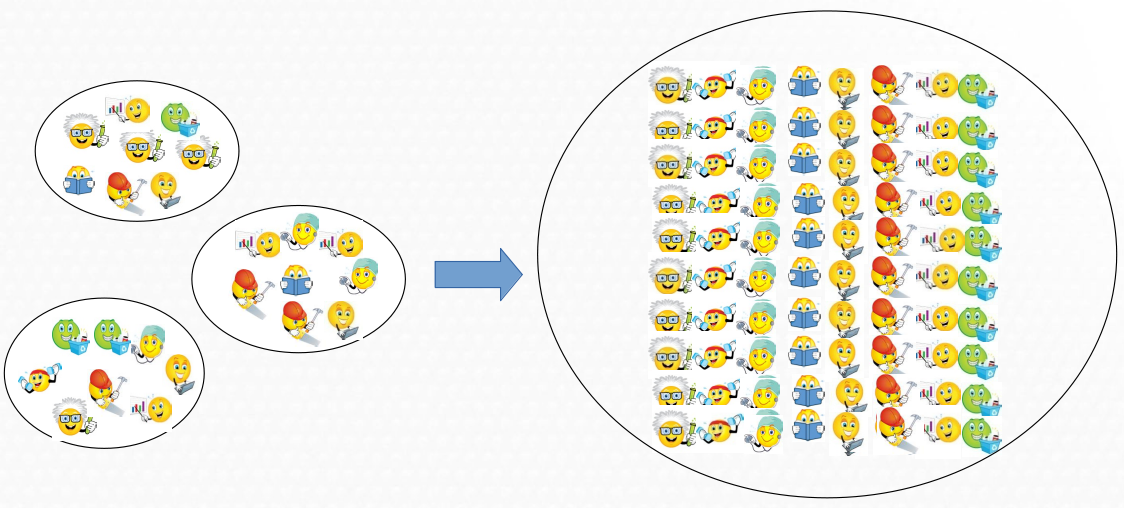
\includegraphics[width=0.8\linewidth]{images/statisticalinference1} \end{figure}

we aim at determining the properties of the entire population.
\end{frame}

\begin{frame}{The objectives of Statistical Inference (II)}
\protect\hypertarget{the-objectives-of-statistical-inference-ii}{}
\begin{figure}
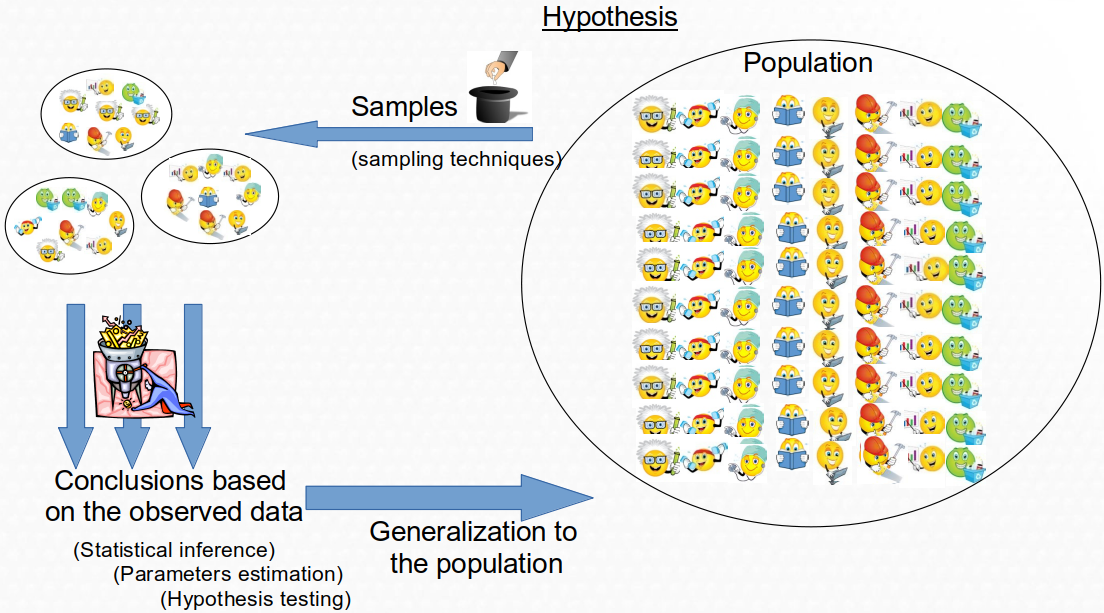
\includegraphics[width=0.8\linewidth]{images/statisticalinference2} \end{figure}
\end{frame}

\begin{frame}{Example}
\protect\hypertarget{example}{}
\begin{itemize}
\tightlist
\item
  Consider the data in the ``osteoporosis.csv'' dataset.
\item
  It can be useful to provide information such as:

  \begin{itemize}
  \tightlist
  \item
    The percentage of menopausic women with osteoporosis
  \item
    The mean bone density in menopausic or non-menopausic women
  \item
    The existence of significance differences:

    \begin{itemize}
    \tightlist
    \item
      Observed \% of osteoporosis vs ``theoretical'' population values
    \item
      BUA in menopasuic vs non menopausic
    \end{itemize}
  \end{itemize}
\item
  Answering these questions (and questions like these) is the main goal
  of Statistical Inference
\end{itemize}
\end{frame}

\begin{frame}{Two types of statistical inference problems}
\protect\hypertarget{two-types-of-statistical-inference-problems}{}
\begin{itemize}
\item
  ESTIMATION

  \begin{itemize}
  \tightlist
  \item
    When we wish to \emph{learn some characteristics of our population},
    such as

    \begin{itemize}
    \tightlist
    \item
      The percentage of non osteopenic or menopausic women
    \item
      The mean bone density in each of these groups
    \end{itemize}
  \end{itemize}
\item
  HYPOTHESIS TESING

  \begin{itemize}
  \tightlist
  \item
    When we wish to \emph{check about some statement on some
    characteristic of the population} or we \emph{wish to make some
    comparisons}

    \begin{itemize}
    \tightlist
    \item
      Is it true that the mean bone density is smaller than 75 in
      menopausic
    \item
      Can we state that non menopausic women have a higher bone density
      than menopausic?
    \end{itemize}
  \end{itemize}
\end{itemize}
\end{frame}

\begin{frame}{Estimators: Aproximating the value of population
parameters}
\protect\hypertarget{estimators-aproximating-the-value-of-population-parameters}{}
\begin{itemize}
\item
  Numerical values calculated on a sample that we believe to be a good
  approximation of a certain real value (parameter) in the population.
\item
  Intuitively, we work with many estimators, such as the mean or a
  computed percentage of a given sample, that we assume that are somehow
  characterizing a population.
\item
  It is \textbf{not always obvious to decide which is the best estimator
  for each parameter}
\item
  In order to decide which estimator we use we can rely on the
  \emph{properties} of the estimators such as \textbf{the bias} or the
  \textbf{precision (the variance)} of the estimator.
\end{itemize}
\end{frame}

\begin{frame}[fragile]{Example. Computing estimations (1)}
\protect\hypertarget{example.-computing-estimations-1}{}
\begin{itemize}
\tightlist
\item
  Read the Osteoporosis dataset and turn factors into variables
  automatically with Rbase function \texttt{read.delim}
\item
  Take a sample of size 100 from the original file. Call it `osteo100'
  and work with this file from now on.
\item
  Compute the mean value of the variable containing bone density values
  \texttt{BUA}
\item
  Split the computation between all subgroups from variable
  \texttt{classific} and variable \texttt{menop}
\item
  Compute the percentage of menopausic women from variable
  \texttt{menop}
\end{itemize}
\end{frame}

\begin{frame}[fragile]{Example. Computing estimations with R (1)}
\protect\hypertarget{example.-computing-estimations-with-r-1}{}
\small

\begin{Shaded}
\begin{Highlighting}[]
\FunctionTok{library}\NormalTok{(dplyr)}
\CommentTok{\# Read data}
\NormalTok{osteoporosis }\OtherTok{\textless{}{-}} \FunctionTok{read.delim2}\NormalTok{(}\StringTok{"datasets/osteoporosis.csv"}\NormalTok{, }\AttributeTok{stringsAsFactors=}\ConstantTok{TRUE}\NormalTok{)}
\CommentTok{\# Take subsample}
\NormalTok{osteo100 }\OtherTok{\textless{}{-}} \FunctionTok{sample\_n}\NormalTok{(osteoporosis, }\DecValTok{100}\NormalTok{)}
\CommentTok{\# mean bone density}
\NormalTok{buaMean }\OtherTok{\textless{}{-}} \FunctionTok{mean}\NormalTok{(osteo100}\SpecialCharTok{$}\NormalTok{bua)}
\FunctionTok{print}\NormalTok{(buaMean)}
\end{Highlighting}
\end{Shaded}

\begin{verbatim}
## [1] 74.23
\end{verbatim}
\end{frame}

\begin{frame}[fragile]{Example. Computing estimations with R (2)}
\protect\hypertarget{example.-computing-estimations-with-r-2}{}
\small

\begin{Shaded}
\begin{Highlighting}[]
\CommentTok{\# Mean bone density ny groups}
\NormalTok{osteo100 }\SpecialCharTok{\%\textgreater{}\%} 
  \FunctionTok{group\_by}\NormalTok{(menop) }\SpecialCharTok{\%\textgreater{}\%} 
  \FunctionTok{summarize}\NormalTok{(}\AttributeTok{m =} \FunctionTok{mean}\NormalTok{(bua))}
\end{Highlighting}
\end{Shaded}

\begin{verbatim}
## # A tibble: 2 x 2
##   menop     m
##   <fct> <dbl>
## 1 NO     84.2
## 2 SI     70.4
\end{verbatim}

\begin{Shaded}
\begin{Highlighting}[]
\CommentTok{\# Proportion of menop women (Proportion  is a mean of 0{-}1 values)}
\FunctionTok{mean}\NormalTok{(}\FunctionTok{ifelse}\NormalTok{(osteo100}\SpecialCharTok{$}\NormalTok{menop}\SpecialCharTok{==}\StringTok{"SI"}\NormalTok{,}\DecValTok{1}\NormalTok{,}\DecValTok{0}\NormalTok{))}
\end{Highlighting}
\end{Shaded}

\begin{verbatim}
## [1] 0.72
\end{verbatim}
\end{frame}

\begin{frame}{Exercise 1}
\protect\hypertarget{exercise-1}{}
\begin{itemize}
\tightlist
\item
  Read the diabetes dataset. Convert characters into factors before
  continuing.
\item
  Provide an estimate of

  \begin{itemize}
  \tightlist
  \item
    The distribution of a numerical variable.
  \item
    a proportion of at least one categorical variable and
  \item
    the mean value of at least one numerical variable.
  \end{itemize}
\item
  Could you have used different estimators?
\item
  How would you decide?
\end{itemize}
\end{frame}

\begin{frame}{How precise is an estimator?}
\protect\hypertarget{how-precise-is-an-estimator}{}
\begin{itemize}
\tightlist
\item
  We all are familar with ``forks'' associated with voting results.

  \begin{itemize}
  \tightlist
  \item
    They usually start ``wide'' and tend to disappear as more votes are
    counted.
  \end{itemize}
\item
  Imagine you are given an estimate of 18\% for the incidence of a
  certain disease.
\item
  Is it a good estimate?
\item
  Hard to know without more information

  \begin{itemize}
  \tightlist
  \item
    \(18 \pm 2%
    \) is probably useful
  \item
    \(18 \pm 12%
    \) is probably too wide to be considered useful
  \end{itemize}
\item
  So given an estimator and a n estimation (a value) \textbf{how can we
  provide a measure of how precise this estimation is}?
\end{itemize}
\end{frame}

\begin{frame}{The \emph{Standard Error} of an estimator}
\protect\hypertarget{the-standard-error-of-an-estimator}{}
\begin{itemize}
\item
  An obvious question when we choose an estimator is \emph{how precise
  it is to approximate the value of the population parameter}.
\item
  This can be answered using the \textbf{standard error of the
  estimator}
\item
  The standard error is a great quantity :

  \begin{itemize}
  \tightlist
  \item
    It informs about the \emph{precision} of our estimates
  \item
    Helps build another type of estimators: \emph{confidence intervals}
  \item
    Helps find formulae to compute \emph{sample size} for estimation
  \end{itemize}
\end{itemize}
\end{frame}

\begin{frame}{Some standard errors}
\protect\hypertarget{some-standard-errors}{}
\begin{itemize}
\tightlist
\item
  Standard error of the sample mean \[
  SEM = \frac{\hat s}{\sqrt{n}}
  \]
\item
  Standard error of the sample proportion \[
  SEP = \sqrt{\frac{\hat p (1-\hat p)}{n}}
  \]
\end{itemize}
\end{frame}

\begin{frame}[fragile]{Computing the standard error with R}
\protect\hypertarget{computing-the-standard-error-with-r}{}
\begin{itemize}
\item
  R does not include functions for standard errors, although it can be
  easily programmed.
\item
  First create the functions
\end{itemize}

\small

\begin{Shaded}
\begin{Highlighting}[]
\NormalTok{SEM }\OtherTok{\textless{}{-}} \ControlFlowTok{function}\NormalTok{ (x)\{}\FunctionTok{sd}\NormalTok{(x)}\SpecialCharTok{/}\FunctionTok{sqrt}\NormalTok{(}\FunctionTok{length}\NormalTok{(x))\}}

\NormalTok{SEP }\OtherTok{\textless{}{-}} \ControlFlowTok{function}\NormalTok{ (x)\{}
\NormalTok{  ssize }\OtherTok{\textless{}{-}} \FunctionTok{length}\NormalTok{(x)}
\NormalTok{  p }\OtherTok{\textless{}{-}} \FunctionTok{sum}\NormalTok{(x)}\SpecialCharTok{/}\NormalTok{ssize}
  \FunctionTok{return}\NormalTok{(}\FunctionTok{sqrt}\NormalTok{(p}\SpecialCharTok{*}\NormalTok{(}\DecValTok{1}\SpecialCharTok{{-}}\NormalTok{p)}\SpecialCharTok{/}\NormalTok{ssize))}
\NormalTok{\}}
\end{Highlighting}
\end{Shaded}

\begin{itemize}
\tightlist
\item
  Then apply them to your data
\end{itemize}

\begin{Shaded}
\begin{Highlighting}[]
\FunctionTok{SEM}\NormalTok{ (osteo100}\SpecialCharTok{$}\StringTok{"bua"}\NormalTok{)}
\end{Highlighting}
\end{Shaded}

\begin{verbatim}
## [1] 1.687018
\end{verbatim}

\begin{Shaded}
\begin{Highlighting}[]
\NormalTok{intMenop }\OtherTok{\textless{}{-}} \FunctionTok{ifelse}\NormalTok{(osteo100}\SpecialCharTok{$}\StringTok{"menop"}\SpecialCharTok{==}\StringTok{"SI"}\NormalTok{, }\DecValTok{1}\NormalTok{, }\DecValTok{0}\NormalTok{)}
\FunctionTok{SEP}\NormalTok{ (intMenop)}
\end{Highlighting}
\end{Shaded}

\begin{verbatim}
## [1] 0.04489989
\end{verbatim}
\end{frame}

\begin{frame}{Confidence intervals}
\protect\hypertarget{confidence-intervals}{}
\begin{itemize}
\tightlist
\item
  Confidence intervals are based on standard errors
\end{itemize}

\begin{figure}
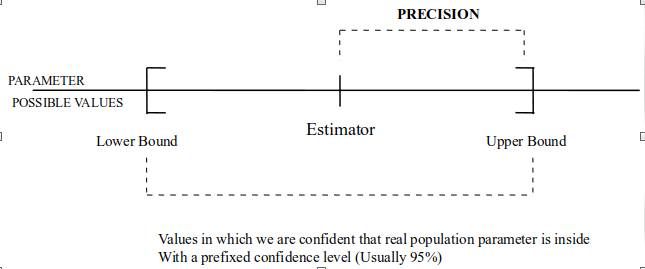
\includegraphics[width=0.8\linewidth]{images/confidenceintervals1} \end{figure}
\end{frame}

\begin{frame}{Formulae for confidence intervals}
\protect\hypertarget{formulae-for-confidence-intervals}{}
\begin{itemize}
\tightlist
\item
  Confidence interval for the mean
\end{itemize}

\[
\overline{X} - \underbrace{t_{\epsilon/2} \frac{\hat s}{\sqrt{n}}}_{Precision} \leq \mu \leq
\overline{X} + t_{\epsilon/2} \frac{\hat s}{\sqrt{n}} = 
\mathbf{\overline{X} \pm t_{\epsilon/2} \cdot \mbox{SEM}}
\]

\begin{itemize}
\tightlist
\item
  Confidence interval for the proportion
\end{itemize}

\[
\hat {p} - \underbrace{z_{\epsilon/2} \sqrt{\frac{\hat p (1-\hat p)}{n}}}_{Precision} \leq \mu \leq
\hat {p} + z_{\epsilon/2} \sqrt{\frac{\hat p (1-\hat p)}{n}} = 
\mathbf{\hat {p} \pm z_{\epsilon/2} \cdot \mbox{SEM}}
\]
\end{frame}

\begin{frame}[fragile]{Example 2. Computing Confidence Intervals with R}
\protect\hypertarget{example-2.-computing-confidence-intervals-with-r}{}
\begin{itemize}
\item
  In general R does not compute (has no functions) for the direct
  calculation of confidence intervals
\item
  This can be done by calling the corresponding tests functions such as
  \texttt{t.test} or \texttt{prop.test}
\item
  Some R commander plugins such as EZR allow this computations directly
\end{itemize}
\end{frame}

\begin{frame}[fragile]
\begin{block}{Example 2. Computing Confidence Intervals with R (2)}
\protect\hypertarget{example-2.-computing-confidence-intervals-with-r-2}{}
\begin{Shaded}
\begin{Highlighting}[]
\FunctionTok{t.test}\NormalTok{(osteo100[[}\StringTok{"bua"}\NormalTok{]])}
\end{Highlighting}
\end{Shaded}

\begin{verbatim}
## 
##  One Sample t-test
## 
## data:  osteo100[["bua"]]
## t = 44.001, df = 99, p-value < 2.2e-16
## alternative hypothesis: true mean is not equal to 0
## 95 percent confidence interval:
##  70.88259 77.57741
## sample estimates:
## mean of x 
##     74.23
\end{verbatim}
\end{block}
\end{frame}

\begin{frame}[fragile]
\begin{block}{Example 2 . Computing Confidence Intervals with R (3)}
\protect\hypertarget{example-2-.-computing-confidence-intervals-with-r-3}{}
\begin{Shaded}
\begin{Highlighting}[]
\NormalTok{cntMenop }\OtherTok{\textless{}{-}} \FunctionTok{table}\NormalTok{(osteo100[[}\StringTok{"menop"}\NormalTok{]])[}\StringTok{"SI"}\NormalTok{]}
\NormalTok{ssize }\OtherTok{\textless{}{-}} \FunctionTok{length}\NormalTok{(osteo100[[}\StringTok{"menop"}\NormalTok{]])}
\FunctionTok{prop.test}\NormalTok{ (}\AttributeTok{x=}\NormalTok{cntMenop, }\AttributeTok{n=}\NormalTok{ssize)}
\end{Highlighting}
\end{Shaded}

\begin{verbatim}
## 
##  1-sample proportions test with continuity correction
## 
## data:  cntMenop out of ssize, null probability 0.5
## X-squared = 18.49, df = 1, p-value = 1.708e-05
## alternative hypothesis: true p is not equal to 0.5
## 95 percent confidence interval:
##  0.6198592 0.8029601
## sample estimates:
##    p 
## 0.72
\end{verbatim}
\end{block}
\end{frame}

\begin{frame}{Exercise 2.1 Computing Confidence intervals}
\protect\hypertarget{exercise-2.1-computing-confidence-intervals}{}
\begin{itemize}
\item
  Read the file ``osteoporosis.csv'' into a dataset and call it
  ``osteoporosis''
\item
  Compute confidence intervals for the BUA mean and for the percentage
  of menopausic women with \textbf{all the individuals in the dataset}.
\item
  Compare these confidence intervals with those that you obtained in
  example 2. How do they differ?
\end{itemize}
\end{frame}

\begin{frame}{Exercise 2.2 Computing Confidence intervals}
\protect\hypertarget{exercise-2.2-computing-confidence-intervals}{}
\begin{itemize}
\item
  Read the diabetes dataset. Convert characters into factors before
  continuing.
\item
  Provide a confidence interval for:

  \begin{itemize}
  \tightlist
  \item
    a proportion of at least one categorical variable and
  \item
    the mean value of at least one numerical variable.
  \end{itemize}
\item
  How would you find alternative approaches to compute these confidence
  intervals?
\item
  Why would you want to do such a thing?
\end{itemize}
\end{frame}

\begin{frame}{Sample Size for estimation (1)}
\protect\hypertarget{sample-size-for-estimation-1}{}
\begin{itemize}
\tightlist
\item
  The standard error informs of how precise an estimation is \textbf{if
  one knows the variability and the sample size}
\end{itemize}

\[
SE =\frac{ \hat \sigma}{\sqrt{n}}
\]

\begin{itemize}
\item
  We can proceed in the opposite sense: assuming we know:

  \begin{enumerate}
  [(1)]
  \tightlist
  \item
    the variability (e.g.~from a pilot study) and
  \item
    the highest precision we wish to attain (``arm length'' of a
    confidence interval:
  \end{enumerate}

  \[
     \Delta = z_{\epsilon_2} \cdot SE = z_{\epsilon_2} \cdot \frac{ \hat \sigma}{\sqrt{n}}
     \]
\end{itemize}
\end{frame}

\begin{frame}{Sample Size for estimation (2)}
\protect\hypertarget{sample-size-for-estimation-2}{}
\begin{itemize}
\tightlist
\item
  The sample size needed to attain this precision can be isolated from
  the previous equation:
\end{itemize}

\[
n= \frac{z_{\epsilon_2} ^2 \hat  \sigma ^2}{\Delta^2}
\]
\end{frame}

\begin{frame}{Sample size formulae for estimating a mean or a
proportion}
\protect\hypertarget{sample-size-formulae-for-estimating-a-mean-or-a-proportion}{}
The previous formula becomes, for specific questions:

\[
n= \frac{t_{n-1, \epsilon_2} ^2 \, \hat  s ^2}{\Delta^2} \quad (1), \qquad 
n= \frac{z_{\epsilon_2} ^2 \, \hat  p (1-\hat p)}{\Delta^2} \quad(2), \qquad 
n= \frac{z_{\epsilon_2} ^2 }{4\,\Delta^2} \quad(3) 
\]

\begin{enumerate}
\item
  Mean of a normal population with a given precision \(\Delta\).
\item
  Proportion \(p\), with a given precision \(\Delta\) and with an
  estimate, \(\hat p\) available, from a pilot study.
\item
  Proportion \(p\), with a given precision \(\Delta\) and assuming the
  \emph{worst case} \(p=q=0.5\).
\end{enumerate}
\end{frame}

\begin{frame}[fragile]{Sample size calculations with R}
\protect\hypertarget{sample-size-calculations-with-r}{}
\begin{itemize}
\item
  There are many packages in R to compute sample size \emph{for
  hypothesis testing}. This means thay have to account not only for
  ``precision'', ``variability'' and ``confidence'', but also with
  ``power''.
\item
  For the sake of examples it is straightforward to write simple
  functions to compute sample size.
\end{itemize}

\begin{Shaded}
\begin{Highlighting}[]
\NormalTok{ssize4Mean }\OtherTok{\textless{}{-}} \ControlFlowTok{function}\NormalTok{ (epsilon, sigma, precision)\{}
\NormalTok{  perc }\OtherTok{\textless{}{-}} \FunctionTok{qnorm}\NormalTok{ (}\DecValTok{1}\SpecialCharTok{{-}}\NormalTok{epsilon}\SpecialCharTok{/}\DecValTok{2}\NormalTok{)}
\NormalTok{  n }\OtherTok{\textless{}{-}}\NormalTok{ ((perc}\SpecialCharTok{*}\NormalTok{sigma)}\SpecialCharTok{/}\NormalTok{prec)}\SpecialCharTok{*}\DecValTok{2}
\NormalTok{\}}
\end{Highlighting}
\end{Shaded}
\end{frame}

\begin{frame}{Example 3. Sample size calculation}
\protect\hypertarget{example-3.-sample-size-calculation}{}
\begin{itemize}
\item
  Using the osteoporosis dataset, assume that the standard deviation is
  a good aproximation to \(\sigma\).
\item
  Find the sample size needed to achieve a margin of error equal to 5
  with a \(95\%\) confidence interval.
\end{itemize}
\end{frame}

\begin{frame}{Exercise 3. Sample size calculation}
\protect\hypertarget{exercise-3.-sample-size-calculation}{}
\begin{itemize}
\item
  Write a function to compute the sample size for proportions in the
  worst case (p=q=0.5) or assuming \(p\) is known.
\item
  Using a \(50\%\) planned proportion estimate, find the sample size
  needed to achieve \(5%
  \) margin of error for a survey at \(95%
  \) confidence level.
\item
  How would this result change if we are told that a pilot study
  suggests that \(p=10\%\)?
\end{itemize}
\end{frame}

\end{document}
